%%%%%%%%%%%%%%%%%%%%%% The Thesis %%%%%%%%%%%%%%%%%%%%%%%%%%%%%%%%%%%%%%%%%%%%%

%%==================== Document Class =======================================%%
% Document class, adjust for different printing/PDF creation modes
\documentclass[oneside,a4paper,12pt]{book}
%\documentclass[twoside,a4paper,11pt,draft]{book}

%%==================== Document Info ========================================%%
\newcommand{\tname}{Lydia Drabsch}
\newcommand{\tdegrees}{BE (Hons 1)}  % optional - define to put degree(s) on title page
% Comment on degrees: Since a thesis is an academic document you probably should
% put your previous degrees after your name, regardless of where they are from.
% The convention is that if a degree is not from your current university you
% should include the abbreviated name of the awarding university. There are
% lists of standard abbreviations of university names (where?). By convention
% you do not put the discipline area, only the degree. For example,
% Tariq Abuhahsim BSc (Uni Name), MSc (Uni Name)
\newcommand{\ttitle}{Instantaneous Relative Positioning of Multiple GPS Receivers}
\newcommand{\tdoctype}{PhD Thesis}
%\newcommand{\tdepartment}{Australian Centre for Field Robotics}
\newcommand{\tschool}{School of Aerospace, Mechanical and Mechatronic Engineering}
\newcommand{\tinstitution}{The University of Sydney}
\newcommand{\tdegree}{Bachelor of Mechatronics (Space) Engineering/Bachelor of Science}
\newcommand{\tdateSubmitted}{8 June 2017}
\newcommand{\tmonthAndYearSubmitted}{June 2017}
% Define the following two when you are creating the final post-examination version
%\newcommand{\tdateRevised}{22 July 2013}
%\newcommand{\tmonthAndYearRevised}{July 2013}
\newcommand{\tkeywords}{your, keywords, go, here}

%%==================== Citation and Reference Style =========================%%
% Choose a reference style from: {apa-like, ieee} or adjust natbib and
% bibliography settings yourself if you prefer something else.
%\newcommand{\tReferenceStyle}{ieee}

%%==================== Included Packages ====================================%%
% If you need to include extra packages, put them into this file; you may want
% or need to remove some packages from the list if conflicts arise from those
% you add.
\input{LaTeX/packages}
%\usepackage{subfigure}
%%==================== Document Layout ======================================%%
% This defines a variety of internal latex whitespace lengths (line spacing,
% margins, magic numbers for automatic layout of floating environments). You
% may need to modify this slightly depending on how you're binding the
% document, and whether you print single or double sided.
%!TEX root = ../Thesis.tex

%%================= Page Layout ======================%%
% Page Layout
\setlength{\topmargin}{0cm}
\setlength{\textheight}{624pt}
\setlength{\textwidth}{6in}
\raggedbottom

% use these for two sided (even on left)
\setlength{\oddsidemargin}{0.0in}
\setlength{\evensidemargin}{0.267in}
% use this for one sided printing with thick left margin
%\setlength{\oddsidemargin}{0.4in}

\setlength{\columnwidth}{\textwidth}
\setlength{\footskip}{0.3in}
\setlength{\headheight}{16pt}                       % todo --- apparently 15pt is the minimum (?)

% Paragraph Layout
\setlength{\parindent}{0em}                         % paragraph indent --- I prefer a space between paragraphs to indents
\setlength{\parskip}{1.5ex plus0.5ex minus0.5ex}    % space after paragraph (rubber length)
\renewcommand{\baselinestretch}{1.4}                % line spacing

% Float Settings
% When using defaults, latex produces many pages with stand-alone figures.
% These settings are meant to improve this a bit; feel free to fiddle with 
% them depending on the sizes and quantity of floating environments you use
\renewcommand{\topfraction}{0.85}
\renewcommand{\bottomfraction}{0.85}
\renewcommand{\textfraction}{0.2}
\renewcommand{\floatpagefraction}{0.2}
\setcounter{topnumber}{2}
\setcounter{bottomnumber}{2}
\setcounter{totalnumber}{4}

%%================= Misc Global Settings =============%%
% how far down section numbers go (chapter/section/subsection/subsubsection/paragraph...)
\setcounter{secnumdepth}{2}

% how far down the TOC goes (chapter/section/subsection/subsubsection...)
%\setcounter{tocdepth}{2}

% Allow pagebreaks in equations
% Currently set to 1 = "if they absolutely must" (see amsmath documentation for more info)
\allowdisplaybreaks[1]



%%==================== Local Package Includes ===============================%%
% Some macros and environment definitions that are used in the template are in
% here. Add your own, either by modifying commands.tex or \input{}ing your own
% tex file.
\input{LaTeX/commands}

%%==================== Document Start =======================================%%
% Document starts here! Everything before this is just configuration...
\begin{document}

%%==================== Setup for Headers for Chapters =======================%%
% Chapter headers are slightly different from the headers in the front matter.
\pagestyle{fancyplain}
\renewcommand{\chaptermark}[1]{\markboth{#1}{#1}}
\renewcommand{\sectionmark}[1]{\markright{\thesection\ #1}}
\lhead[\fancyplain{}{\thepage}]{\fancyplain{}{\nouppercase\rightmark}}
\rhead[\fancyplain{}{\nouppercase\leftmark}]{\fancyplain{}{\thepage}} \cfoot{}

%%==================== Front Matter =========================================%%
% Everything prior to chapter 1
%!TEX root = ../Thesis.tex

% FrontMatter.tex
% This file contains no real content, just commands to generate/include the various sections of the
% pages before Page 1 of Chapter 1 (the Introduction).

% Macro to generate most front-matter-sections
%\frontsec{title}{heading=none,centred,normal}{content}
\newcommand{\frontsec}[3]{
    \cleardoublepage% each section starts on a new page (RHS page if doublesided)
    \phantomsection% required for hyperrefs to work properly to subsequent contents line
    \addcontentsline{toc}{chapter}{#1}% TOC entry
    \begin{singlespace}% most of the front matter can be single spaced
        % Optional headings (some content provides its own, e.g. \tableofcontents)
        \ifthenelse{\equal{#2}{none}}{%
            % no headings required
        }{% else
            % heading required (normal / centred)
            \chapter*{\ifthenelse{\equal{#2}{centred}}{\centering}{} #1}%
            % and page headers too, seems to be attached to whether or not the content generates its
            % own heading
            \markboth{#1}{#1}%
        }%
        % Content
        #3%
    \end{singlespace}%
}%

% Title page
\pagenumbering{Roman} % to prevent duplicate page number issues with the *real* page 1
%!TEX root = ../Thesis.tex

% Produce the title page
\thispagestyle{empty}

\begin{center}
  \begin{Huge}

  {\bf
    \ttitle \\
  }
  \end{Huge}

  \vfill

  \begin{large}
  {\bf
    \ifdefined\tdegrees
        \tname \enspace \tdegrees
    \else
        \tname
    \fi
  }
  \end{large}

  \vfill% expand this space to fill the page nicely

  A thesis submitted in fulfillment\\
  of the requirements of the degree of\\
  \tdegree{}

  \vspace{0.50cm}

  % NOTE that USyd policy states that the crest should ONLY appear on a thesis
  % once it has been examined and passed. This is because the use of the crest
  % could be taken by an examiner to imply University endorsement of the thesis.
  % Your initial drafts and submissions should not include the crest.

  % If printed in colour, use colour logo.
  
\includegraphics[width=4cm]{FrontMatter/Figures/USYD_Logo_Colour_Stacked.pdf}     % min width = 2.0cm
  %
\includegraphics[width=6.4cm]{FrontMatter/Figures/USYD_Logo_Colour.pdf}           % min width = 3.2cm

  % If printed in grayscale (or to be photocopied), use the black and white logo.
  %
\includegraphics[width=4cm]{FrontMatter/Figures/USYD_Logo_Black_Stacked.pdf}      % min width = 2.0cm
  %
\includegraphics[width=6.4cm]{FrontMatter/Figures/USYD_Logo_Black.pdf}            % min width = 3.2cm

  \vspace{0.50cm}

  {
%      \tdepartment{}\\
      \tschool{}\\
      \tinstitution{}\\
  }
  \vspace{0.50cm}

  \begin{center}
    \ifdefined\tmonthAndYearRevised
        % for final emended/corrected version:
        Submitted \tmonthAndYearSubmitted; revised \tmonthAndYearRevised
    \else
        % for version submitted for examination:
        \tmonthAndYearSubmitted
    \fi
  \end{center}


\end{center}


% Roman page numbering for the Front Matter pages
\clearpage{\pagestyle{empty}\cleardoublepage}
\pagenumbering{roman}

% Declaration (bit dodgy - not single spaced like the rest)
\frontsec{Declaration}{normal}{\begin{onehalfspace}%!TEX root = ../Thesis.tex

I hereby declare that this submission is my own work and that, to the best of my knowledge and
belief, it contains no material previously published or written by another person nor material which
to a substantial extent has been accepted for the award of any other degree or diploma of the
University or other institute of higher learning, except where due acknowledgement has been made in
the text.

\vspace{3cm}
\textbf{\tname}

\vspace{1cm}
\ifdefined\tdateRevised
    % for final emended/corrected version:
    \tdateRevised
\else
    % for version submitted for examination:
    \tdateSubmitted
\fi

\end{onehalfspace}}

% Abstract, Acknowledgements as normal
\frontsec{Abstract}{centred}{%!TEX root = ../Thesis.tex

% remove spacing after the "Abstract" heading (looks awkward, and wastes space)
\vspace{-2.5em}

% Sometimes it's worth changing the spacing a little to make it fit nicely on the page, or % have paragraphs fit nicely. Don't go overboard, but 0.95 to 1.4 may be acceptable.

\begin{spacing}{1.1}

    Abstract text goes here\dots{}

    If you've just opened up this template, you should check out \autoref{ch:intro} for a quick introduction. Note also that hyperlinks are rendered in colour for convenience during editing---see ../LaTeX/packages.tex. Note also that there is a simple way to change all of the coloured hyperlinks to black in ../LaTeX/packages.tex---look for \texttt{\textbackslash{}usepackage[colorlinks}.

    \textcolor{highlightcolor}{This paragraph is coloured in ``highlightcolour'', defined in ../LaTeX/commands.tex. To get rid of all highlighting in the document you can just redefine highlightcolour---see \texttt{\textbackslash{}definecolor{highlightcolor}} in  ../LaTeX/commands.tex. Also have a look at \texttt{\textbackslash{}definecolor\{todocolour\}} and \texttt{\textbackslash{}definecolor\{TODOcolour\}} in the same file.}
    
    Lorem ipsum dolor sit amet, consectetur adipisicing elit, sed do eiusmod tempor incididunt ut
    labore et dolore magna aliqua. Ut enim ad minim veniam, quis nostrud exercitation ullamco
    laboris nisi ut aliquip ex ea commodo consequat. Duis aute irure dolor in reprehenderit in
    voluptate velit esse cillum dolore eu fugiat nulla pariatur. Excepteur sint occaecat cupidatat
    non proident, sunt in culpa qui officia deserunt mollit anim id est laborum.

    Lorem ipsum dolor sit amet, consectetur adipisicing elit, sed do eiusmod tempor incididunt ut labore
    et dolore magna aliqua. Ut enim ad minim veniam, quis nostrud exercitation ullamco laboris nisi ut
    aliquip ex ea commodo consequat. Duis aute irure dolor in reprehenderit in voluptate velit esse
    cillum dolore eu fugiat nulla pariatur. Excepteur sint occaecat cupidatat non proident, sunt in
    culpa qui officia deserunt mollit anim id est laborum.


\end{spacing}

}
\frontsec{Acknowledgements}{normal}{%!TEX root = ../Thesis.tex

% Acknowledgements text

\begin{spacing}{1.0}
    Thank you to my supervisor for his patience and understanding.\\
    Thank you to my parents Kathy and Brian, who kept my sanity safe while I wasn't using it.   
\end{spacing}
}

% Dedication (no headings or ToC entry, so just input bare)
\newpage
\begin{singlespace}
    %!TEX root = ../Thesis.tex

\thispagestyle{empty}

\vspace*{\fill}

\begin{flushright}
You could dedicate the thesis to someone, or write something poignant\dots

% Dedication text

    \emph{Hydrogen, in sufficient quantity and given enough time,\\
        will end up writing, reviewing and hopefully citing this thesis.}
 \end{flushright}

\vspace*{\fill}


\end{singlespace}

% Lists/Tables of chapters&sections, figures, tables, algorithms, examples, ...
%\fancyhead[R]{\nouppercase{\rightmark}}
%\fancyhead[R]{\nouppercase{\leftmark}}
\frontsec{Contents}{none}{\tableofcontents}
\frontsec{List of Figures}{none}{\listoffigures}
\frontsec{List of Tables}{none}{\listoftables}
\frontsec{List of Algorithms}{none}{\listofalgorithms}
\frontsec{List of Theorems}{none}{\def\listtheoremname{List of Theorems}\listoftheorems}

% Nomenclature & Glossary
\frontsec{Nomenclature}{normal}{%!TEX root = ../Thesis.tex

\label{fr:notation}

\def\NomenLHSwidth{2.5cm}
\def\NomenRHSwidth{12.5cm}

\subsection*{List of Symbols}\label{fr:symbols}
    %\setlength{\extrarowheight}{5pt}
    \begin{supertabular}{p{\NomenLHSwidth} p{\NomenRHSwidth}}
        v & Variable Name, units \\
    \end{supertabular}

\subsection*{List of Acronyms}\label{fr:acronyms}
% Convert any \acro commands to \acrodef to hide them from this table
% Use \acused{..} to avoid them being expanded on first use in the text

\begin{acronym}[\hspace{\NomenLHSwidth}\hspace{1em}]
    % This makes the short versions of acronyms displayed here less ugly
    % I'm really not sure why they chose sans-serif!
%    \renewcommand{\bflabel}[1]{\hspace{0.5em}\textbf{#1}\hfill}
    % You can use this \comm to add a comment to acronyms, which is only shown in this list
    % (not when the acronym is expanded)
    % Nicer 'acroextra' text - italics in parens to follow full version for extra description
    % e.g. \acro{ABC}{A Big Company \comm{sometimes known as `AB Co.'}}
    \newcommand{\comm}[1]{\acroextra{ \emph{(#1)}}}
    % Compress the list vertically since its not 'normal' paragraphs of text in a list
    \setlength{\itemsep}{0pt}
    \setlength{\parskip}{0pt}

    % The actual acronym definitions go here.
    % A number of examples are provided that may be useful (they'll only show up if you use them)
    % These demonstrate quite a few of the features of the acronym package, including customising
    %   the abbreviated form, having comments in this list, customising the plural form,
    %   disabling expansion-on-first-use for certain acronyms, and having acronym definitions
    %   refer to other acronyms!
    %
    % Note that is is preferable to capitalise ONLY proper nouns in the definitions.
    \acro{USyd}{University of Sydney}
    \acro{ACFR}{Australian Centre for Field Robotics}
    \medskip
    \acro{UAV}{unmanned aerial vehicle}
    \acro{UGV}{unmanned ground vehicle}
    \acro{AUV}{autonomous underwater vehicle}
    \acro{UxV}{unmanned vehicle\comm{not specific to ground, sea or air}}
    \medskip
    \acro{INS}{inertial navigation system}\acused{INS}
    \acro{GPS}{global positioning system}\acused{GPS}
    \acro{DGPS}{differentially-corrected \acs{GPS}}
    \acro{RTK}{real time kinematic\comm{corrections for \acs{GPS}, similar to \acs{DGPS}}}
    \acro{GPSINS}[GPS/INS]{\acs{GPS} and inertial navigation system}
    \acro{SLAM}{simultaneous localisation and mapping}
    \acro{lidar}{light detection and ranging\comm{also commonly known as `ladar' or a `laser range scanner'}}
    \acrodefplural{lidar}{light detection and ranging}
    \acro{IMU}{inertial measurement unit}
    \medskip
    \acro{DDF}{decentralised data fusion}
    \acro{EM}{expectation maximisation}
    \acro{KF}{Kalman filter}
    \acro{EKF}{extended \acl*{KF}}
    \acro{GP}{Gaussian process}
    \acrodefplural{GP}{Gaussian processes}
    \acro{PF}{particle filter}
    \acro{RRT}{rapidly-exploring random tree}
    \acro{RTFM}{read the fcuking manual}
    \acro{PCA}{principal component analysis}
\end{acronym}

}
\frontsec{Glossary}{normal}{%!TEX root = ../Thesis.tex

% Glossary
% According to the OED, a glossary is "a collection of glosses; a list with 
% explanations of abstruse, antiquated, dialectal, or technical terms; a partial 
% dictionary." Glossary entries should be used to define terms that may be 
% unknown to the reader. They will be particularly useful when a thesis draws 
% from a variety of non-engineering backgrounds such as psychology or geology.

\label{fr:glossary}

% Begin description
\begin{description}

    \item[\LaTeX plugin:]\label{gloss:plugin} A \LaTeX package.
    \item[Term:]\label{gloss:term} This term means stuff.

\end{description}
}

% Now entering the main body of the document ...
\cleardoublepage
\pagenumbering{arabic}
\setcounter{page}{1}



%%==================== Chapters =============================================%%
% Adjust the file names below to point to the main chapter .tex file for each
% chapter, and don't forget to update the relative paths inside the files
% within chapters as you rename directories! All paths are relative to the
% location of THIS file, Thesis.tex.
%!TEX root = ../Thesis.tex

\def\chapdir{./ChapterIntro}

\chapter{Introduction} \label{ch:intro}

%% Stefan Williams::
%Introduction
%1.1 Background and Motivation (General fluff then location and mapping)
%1.2 Problem Summary
%1.3 Principle Contributions
%1.4 Outline

%%=======================================================%%

\section{Background and Motivation}

\section{Problem Summary}

\section{Principle Contributions}

\section{Outline}

epoch synchrosation followed by two fold optimisation process\\
need instantanous relative positioning with minimal calibration or setup of external hardware

Instantaneous Relative displacement/position between GNSS receivers.\\
Simulation case studies are presented to validate the mathematical models.\\

The algorithm presented is designed to replace current methods.

With a local reference point with a well known global location, the relative position of the other receivers 						% Chapter 1
%!TEX root = ../Thesis.tex

\def\chapdir{./ChapterLiteratureReview}

\chapter{Literature Review} \label{ch:litreview}



%\section{Position Requirements}
%- how/why to use position for applications\\
%- absolute vs relative\\
%- why use relative positioning\\
%- knowing where you are positioned is important for data gathering, motion detecting and tracking, path planning\\
%- formation flying, drones\\
%- data fusion, needed for drift correction

%\section{GNSS Introduction} % just have as intro to the lit review?
%America with GPS and Russia with GLONASS are at the time of writing the only two fully functional GNSS constellations. The EU and China are developing their own constellations called Galileo and Beidou respectively.

Global Navigation Satellite System (GNSS) is a generic term for a satellite navigation system that provides autonomous localisation and tracking on a global scale. Some countries have developed or in the process of developing their own GNSS. This thesis focuses on the American GPS (Global Positioning System) due to information accessibly and extensive usage in literature as it is the oldest constellation.

\begin{figure}[!h]
\centering
\caption{GPS Constellation in Earth-Centered Inertial frame}
\label{fig:GPS_ECI_side}
\begin{subfigure}[t]{0.49\linewidth}
\centering
\caption{Side View}
\includegraphics[trim=6cm 9.5cm 6cm 10cm,clip,width=0.8\linewidth]{ChapterLiteratureReview/GPS_ECI_side}
\end{subfigure}
\begin{subfigure}[t]{0.49\linewidth}
\centering
\caption{Top View}
\includegraphics[trim=4cm 10cm 4cm 9cm,clip,width=\linewidth]{ChapterLiteratureReview/GPS_ECI_top}
\end{subfigure}
\end{figure}

%\begin{table}
%\centering
%\caption{GNSS Constellations}
%\label{Table:gnss constellations}
%\begin{tabular}[width=\linewidth]{|l|l|c|c|c|}
%\hline
%Country & Name & Number of Satellites & Start Date & End Date \\\hline
%America& GPS & 31 & &  \\\hline
%Russia & GLONASS & 24 & 1976 &  \\\hline
%European Union& Galileo &  & 1998 & \\\hline
%China & Beidou & & &  \\\hline
%\end{tabular}
%\end{table}

%!TEX root = ../Thesis.tex


\section{GPS Operational Components}
There are three components to the whole GPS system; the space segment, the user segment, and the ground control segment. The satellite sends radio signals towards the Earth which is received by both users and ground control centers. The ground control tracks the satellite and the data to analyse the satellite parameters and returns periodic updates to the satellite about its status. The satellite then updates its signal to the new parameters. The user receives the signal from the satellite with the updated parameters.

\subsection{Space Segment}
A set of satellites in the same network is called a constellation. The GPS constellation consists of 30 active and spare NAVSTAR (NAVigation System with Timing and Ranging) satellites \cite{navpedia_spaceseg}. There are 24 satellites in the nominal configuration of 6 orbits with 4 satellites evenly spaced in the orbit with 90$^\circ$ separation, see Figure \ref{fig:GPS_ECI_side}. Each orbital plane is inclined at 55$^\circ$ and evenly spaced around the Earth with 60$^\circ$ separation. All of the orbits are almost circular with an eccentricity of 0.02 and an altitude (semi-major axis) of 20 200 km. This type of orbital configuration was chosen so that the period of the satellites are half of a sidereal day, 11 hours 58 minutes 2 seconds. With a masking of 15$^\circ$ from the horizon, this configuration provides coverage of a minimum of four satellites for every point on Earth, consistently \cite{understandinggps_ss}. Each satellite sends radio signals towards Earth and receives updates from ground control. The signals are explained more in Section \ref{sec:signals}.
%speed of 3.9 km/s




%http://content.schweitzer-online.de/static/catalog_manager/live/media_files/representation/zd_std_orig__zd_schw_orig/004/372/251/9780890067932_content_pdf_1.pdf
%http://www.gps.gov/systems/gps/space/

\subsection{User Segment}
The user is a passive participant in the GPS system, it receives the radio signals and processes them to determine position, velocity and timing (PVT). There are millions of receivers around the world covering military and civilian applications by ships, aircraft, ground vehicles and individuals.

WHERE TO PUT THIS?\\
Unfortunately, low cost GPS receivers rarely provide official access to the GPS raw data. Previous studies have used customised bluetooth headsets or customised android platform mobile phones to investigate algorithms on low-cost GPS receivers. More expensive receivers do allow raw data to be utilised, however they also provide other mechanisms such as duel frequencies and more accurate clocks, rendering the new algorithm *obtuse*. The mindset of *crowd-sourcing*/customising/flexible technology is changing the way manufactures build GPS receivers. The new Android OS platform Nougat 7.0 provides the developer raw GPS data at the software level.  

\subsection{Ground Control Segment}
On the ground spread all over the world, are control stations that monitor the satellites. The ground stations use the Herrick-Gibbs algorithm to determine the orbit of the satellite. A satellite is tracked over a ground station for a period of time and its position is measured. From three position vectors the velocity vector can be calculated and the ephemeris parameters are estimated. The ephemeris parameters describe the orbit of the satellite and are used to calculate the position of the satellite at any point in time by the user segment. The time parameters and clock corrections of the satellite are also calculated by the ground control station and sent back in the navigation message. The ephemeris data is highly accurate and updated every two hours.






%!TEX root = ../Thesis.tex

\section{GPS Satellite Signals}
The are two frequencies that GPS uses; L1 frequency at 1575.42 MHz and L2 at 1227.60 MHz \cite{postprocessing multi}.

There are two sets of signals that are sent from every satellite, the pseudorandom binary sequence (PRN code) and the navigation message.

\subsection{Course Acquisition Code}
The course acquisition code (C/A) 

Low cost GPS receivers only have access to 

The PRN code is intentionally complex to stop jamming 

L1 frequency of 1575.42 Mhz  - code phase
Course Acquisition (C/A) code is transmitted on the L1 frequency as 1.023 MHz signal using a bi-phase shift keying modulation technique.
Navigation message sent at 50 bits per second  


\subsection{Navigation Message}
The navigation message is a low 

\url{https://ocw.mit.edu/courses/earth-atmospheric-and-planetary-sciences/12-540-principles-of-the-global-positioning-system-spring-2012/lecture-notes/MIT12_540S12_lec7.pdf}

- civilian GNSS using duel frequency, send CDMA, how decryption works\\
- what is psudorange?\\
- what is carrier phase\\
- clock bias\\

\subsection{Raw Data}
There is a lot of data contained in the total signal, but the following are what is important to this thesis:
\begin{itemize}
	\item \textbf{Time received}: The time in the receivers frame that the sample reading was taken.
	\item \textbf{Pseudorange}: The range calculated by the receiver to the satellite. Depending upon the type of receiver, this measurement may have already been adjusted for some errors that were encoded in the navigation message.
	\item \textbf{Carrier Phase}: The phase of the carrier signal at the receivers point in time.
	\item \textbf{Doppler Shift}: The instantaneous Doppler frequency of the signal. 
	\item \textbf{Satellite Epoch}: The time the signal was sent from the satellite, decoded from the navigation message.
	\item \textbf{Ephemeris Data}: The orbital parameters necessary to calculate the position of the satellite.
\end{itemize}


%The first row shows a C/A code with 1,023 chips; the total length is 1 ms. The second row shows a navigation data bit that has a data rate of 50 Hz; thus, a data bit is 20 ms long and contains 20 C/A codes. Thirty data bits make a word that is 600 ms long as shown in the third row. Ten words make a subframe that is 6 seconds long as shown in row four. The fifth row shows a page that is 30 seconds long and contains 5 subframes. Twenty-five pages make a complete data set that is 12.5 minutes long as shown in the sixth row. The 25 pages of data can be referred to as a superframe http://read.pudn.com/downloads85/ebook/326017/Fundamentals%20of%20Global%20Positioning%20System%20Receivers/booktext05.pdf (pg77)

% resources about the signals:
% http://geoconnect.com.au/gps-signals-l1-l2-l5/
% http://www.trimble.com/gps_tutorial/dgps-advanced4.aspx
% https://www.e-education.psu.edu/natureofgeoinfo/c5_p14.html
% http://what-when-how.com/gps/gps-details/
% https://www.e-education.psu.edu/geog862/node/1742
% https://ocw.mit.edu/courses/earth-atmospheric-and-planetary-sciences/12-540-principles-of-the-global-positioning-system-spring-2012/lecture-notes/MIT12_540S12_lec7.pdf
% http://read.pudn.com/downloads85/ebook/326017/Fundamentals%20of%20Global%20Positioning%20System%20Receivers/booktext05.pdf
% http://www.navipedia.net/index.php/GPS_Navigation_Message

%!TEX root = ../Thesis.tex

\section{Trilateration}
Unlike triangulation, which uses the angles from known points, trilateration uses the distances from known points. This is the base concept behind GNSS. Satellite W sends out a radio signal at time X and it's position Y which the user received at time Z. The time difference is used to calculate the distance from the satellite's position. With this information from multiple satellites, the users position is calculated.



- timing comparison between satellite and receiver to find psudeorange
- ECEF frame of reference

\begin{figure}
\centering
\caption{}
\label{fig:trilateration}
\includegraphics[width=0.7\linewidth]{ChapterLiteratureReview/trilateration}
\end{figure}

\begin{figure}
\centering
\caption{}
\label{fig:trilaterationtime}
\includegraphics[width=0.7\linewidth]{ChapterLiteratureReview/trilaterationtime}
\end{figure}







- NLLS solve spheres
- need 4 satellites minimum
- 


%!TEX root = ../Thesis.tex

\section{GPS Error Sources} \label{sec:error sources}
There are many sources of error that plague the GPS data. These errors are categorised into six types; multipath, atmospheric effects, receiver noise, ephemeris error, clock bias and Sagnac effect.

\subsection{Mutlipath Interference}
Multipath is the case where the radio signal is reflected off objects before reaching the receiver, which increases the distance travelled. It is especially prevalent in built-up areas with tall buildings. 

\subsection{Atmospheric Effects}
The distance from a satellite to a user is calculated by the time difference when the radio signal was sent and when it was received multiplied by the speed of light. However, the speed of light is reduced when in the atmosphere compared to that in space.
The ionosphere is the upper layer of the atmosphere ranging from 50 to 500 km. It consists of ionized particles that create fluctuating electric fields in the atmosphere that perturb the radio signals that travel through it. This effect can be modelled but is still a significant source of error, approximately 5 m \cite{trimble_errors}. The troposphere is the lowest part of the atmosphere up to 50 km that varies in temperature and pressure with weather patterns. The radio signals are refracted through the medium, but as it is only for a short period of time this error is significantly less than that of the ionosphere at approximately 0.5 m error \cite{trimble_errors}.

\subsection{Receiver Noise}
In any electronic components, especially low cost components, thermal noise introduces error into the system. Thermal noise is caused by the random motion of electrons in conducting materials. The construction of the electrical components are not identical, which also cause slightly different solutions from receiver to receiver. This can contribute approximately 0.3 m of error \cite{trimble_errors}.

\subsection{Ephemeris Error}
The ephemeris error is the error in the navigation data describing the orbital parameters of the satellite \cite{Kaplan_ephemeriserror}. This information is approximated and updated every 2-4 hours by the control segment to minimise the error. The approximation is based on a prediction model of the orbital parameters, as there are many forces that act on a satellite that can alter the orbit. These include gravitational affects of other masses in the solar system such as the Moon, the Sun, even Jupiter and the outer planets affect the gravitational potential of objects in orbit around Earth. The non-spherical Earth, solar radiation pressure, slight atmospheric pressure are all forces that manipulate the orbit. The satellites also undergo station keeping manoeuvres to manage the orbit, which the requires the ephemeris data to update. This inaccuracy contributes about 2.5 m in error \cite{trimble_errors}.

\subsection{Clock Bias}
The clock on the satellites and receivers are not exact with the true GPS time. Low-cost receivers are built with cheap quartz crystal oscillators that keep time to $1\mu s$ accuracy. The clocks on the satellites however are atomic clocks that have accuracy on the order of $1 ns$. In addition to this, ground control can measure the satellite clock bias and send back that information to be stored in the navigation message. \cite{zinas_2015}

\subsection{Sagnac Effect}
The sagnac effect is a more intrinsic source of error. It is due to the rotation of the Earth during the time of the signal transmission. The transmission time is between 0.06-0.08 seconds in which time the Earth has rotated approximately 30 m. If the ephemeris data was in an inertial frame (ECI) there would not be a problem. However, the data is in the Earth-Centred Earth-Fixed (ECEF) frame which is a frame that rotates with the Earth to allow users to calculate their positions independent of time \cite{HighAccDiffTrack}.

\subsection{GPS Error Summary}
All of the errors mentioned above can be categorised into three types; satellite correlated, receiver correlated, and uncorrelated errors. That is, a particular type of error may be consistent between all receivers from a particular satellite, or consistent between all satellite measurements for a particular receiver, or neither. See Table \ref{Table:error catagory}.

\begin{table}
\centering
\caption{Categorisation of Errors}
\label{Table:error catagory}
\begin{tabular}{|c|c|c|}
\hline
Satellite & Receiver & Uncorrelated \\\hline
satellite clock bias & receiver clock bias & multipath \\
ionospheric delay & receiver noise& Sagnac \\
tropospheric delay & &  \\
ephemeris error & & \\\hline
\end{tabular}
\end{table}

 % DONE

%! TEX root = ../Thesis.tex


\section{Multiple Receivers}
- problems arising with multiple receivers

A single sample of pseudoranges from any two receivers will not be taken at the exact same time without a connecting network to implement control. This means that the satellite positions at the time of each signal transmission will be actually different. The primary issue with calculating the change in pseudorange is identifying the transmission time 


\subsection{Align Reception time}
In \cite{HighAccDiffTrack}, they align the reception time of multiple receivers

They precisely align the epoch by accounting for the differing Sagnac effect between two receivers and accounting for the clock biases of the receivers. The Sagnac effect manifests in the multiple receivers case by the signal propagation time for a measurement taken at $t_2$ would be different than if it was taken at $t_1$, the Earth will have rotated by different amounts. 
\begin{enumerate}
\item The clock bias is calculated by solving for the individual absolute position of a receiver using least squares. This is necessary in order to 
\item  
\end{enumerate}

%!TEX root = ../Thesis.tex

\section{Current GNSS algorithms}
- just reference implementation papers?
- algorithms to make it more accurate\\
- use for motion tracking\\
- performance vs cost trade off\\
(http://ieeexplore.ieee.org.ezproxy1.library.usyd.edu.au/document/7530542/)
\subsection{Standard Positioning Service}
- single frequency and multi frequency to remove atmospheric affects
\subsection{Differential GPS}


- explain what it is\\
- what setup is required \\
- abs vs rel \\
- degree of accuracy
\subsection{WAAS DGPS}

\subsection{SBAS  ?}

\subsection{Real Time Kinematic}

\subsection{Post Processing Algorithm}

\subsection{Single Frequency Precise Point Positioning (SF-PPP)}
Rademakers \textcolor{red}{how to say reference?} at University of Delft in the Netherlands developed a solution for finding the absolute position in open areas to a horizontal accuracy of 0.5 m. It uses a single frequency, single antenna low cost GPS receiver by connecting to the internet and using real time information to model all errors. The errors they corrected with the potential improvements are outlined in Table \ref{Table:SFPPP error table}. 
\begin{table}
\centering
\caption{Error Components and Potential Improvements for SF-PPP}
\label{Table:SFPPP error table}
\begin{tabular}{|l|l|}
\hline
\textbf{Error component} &\textbf{ Potential Improvement} \\\hline
 Ionosphere: Klobuchar model & 7 m \\\hline
 Troposphere: Saastamoinen model & 2.5 m \\\hline
Ephemeris data &  1 m \\\hline
 Satellite clock drift & 1.5 m \\\hline
 Differential code bias & 50 cm \\\hline
 Phase windup: rotation of the antenna & dm \\\hline
 Sagnac effect & 30 m \\\hline
 ROA: satellite orbit correction & up to 10 cm \\\hline
 Relativistic clock correction & up to 21 m \\\hline
 Moon-Earth interaction & 5cm (Hor) and 30 cm (Ver)\\\hline
\end{tabular}
\end{table}


\subsection{Duel-Epoch, Double-Differencing Model} \label{DEDD}
In the paper by the Institute of Software Integrated Systems, Vanderbilt University called \textit{High-Accuracy Differential Tracking of Low-Cost GPS Receivers}, Hedgecock and party developed a new algorithm for relative motion tracking for multiple receivers. They used low cost GPS receivers with access to raw measurement data to produce centimeter-scale tracking accuracy. Each receiver was shared the whole networks data and ran the localisation algorithm independently to avoid having a single point of failure.\\

The algorithm uses the change in carrier phase through time of each receiver to estimate the change in relative ranges between a satellite and two receivers. It does not require a reference satellite, a reference node or an integer ambiguity solution. It does require the clock bias for each receiver at each point in time as solved for by non-linear least squares for the absolute position before running the algorithm itself. To reiterate, it does not directly solve for the relative position but the relative motion. However, neither of the initial positions of the receivers need to be precisely known in order for the relative motion to be accurate. Due to the time dependency, consistent satellite locks of at least four satellites are required, otherwise reinitialisation must occur. The calculated change was projected onto the unit direction vector from receiver to satellite. The system of these tracking equations was solved via least squares optimisation. \\

It uses the assumption that all satellites in the constellation are such a great distance from the surface of the Earth that the unit vector from both receivers are parallel to each individual satellite, as long as it is in the same geographical region. How far apart the receivers can be for this assumption to hold was not stated.\\ 




- how many receivers?\\
- why and how it aligns epoch\\
- uses difference in time for a single receiver to find change in motion.



- have this one last as it is the most similar\\
- needs instantaneous relative distance for first point, to speed up processing and make the first few time steps more accurate, also when locking onto new satellites


\subsection{Summary of Algorithms ?}

% types of algorithms making gps more accurate: table with columns = types of analysis, rows= types of algorithms
- dynamic tracking (need temporal measurements) vs static measurement - no temporal\\
- post processing vs pre-processing vs realtime\\
- ground structure vs free standing\\
- absolute vs relative\\
- accuracy (how much)\\
- computation time/space required\\
- what error is each method removing\\
- what piece of data it needs (if raw)\\
- calibration required\\
- robustness -> if a satellite goes out of view does it need to re-calibrate? passing information between receivers-> is one a reference? single point of failure





%!TEX root = ../Thesis.tex

\section{Moving Forward} % or is it conclusion?
GPS is currently going through a major upgrade, with the launch of new satellites with alternate structuring of signals that will provide greater accuracy for civil use in the future. The constellation Galileo that is currently being developed and launched, is expected to be finished by XX. Both the new GPS and Galileo are designed to be able to operate in tandem to provide an *unprecedented* accuracy with a total of 57 operational joint satellites, while still having the individual capability of global coverage. Some technology today uses both GPS and GLONASS constellations but requires duel receivers as the signals are encoded differently. GPS uses code division multiple access (CMDA) whereas GLONASS uses frequency division multiple access (FMDA). Research is also being conducted on the sources of error in the radio signals. The errors are to be modelled and the appropriate adjustments stored in the encoding of the signal. Through the international cooperation efforts and research, localisation and tracking using baseline GNSS will continue to improve, regardless of alternate data processing algorithms. For now, improved signal accuracy will obviously improve the performance of the different data processing algorithms. However, there will come a time where the extra computational and hardware complexity will not be worth the small gain in accuracy over the default performance of the low-cost civilian GNSS receiver.
 % DONE








%??Topical organisation with inverted pyramid substructure
% \subsection{GNSS Localisation}
% Global Navigation Satellite System (GNSS) 
% - lower update rates $\approx$1Hz\\
% - accuracy/precision? not good enough for these applications\\
% - not good for indoor environments as signals are weak\\
% - used differentiated gnss to solve for integer ambiguity across multiple mobile platforms on the go \cite{GNSS_difftrack} \cite{GNSS_intamb}\\
% - multipath/atmospheric error estimation \\
% - multiple receivers across the multiplayers \cite{GNSS_multi} \\

% 	%% types of precision gnss locations 
% - double differentiating - requires same satellites
% - pvt position velocity and precise time	% Chapter 2
%!TEX root = ../Thesis.tex

\def\chapdir{./ChapterPerception}

\chapter{Example Chapter on `Perception' Stuff}\label{ch:perception}

%%%%%%%%%%%%%%%%%%%% Introduction %%%%%%%%%%%%%%%%%%%



%%%%%%%%%%%%%%%%%%%% Content Sections %%%%%%%%%%%%%%%%%%%


%!TEX root = ../Thesis.tex
\section{Methodology}
The following methodology describes how PA was implemented. 

%https://www.e-education.psu.edu/geog862/node/1759 - errors in pseduorange

%http://www.insidegnss.com/node/2898 - how to get pseudorange from raw data
\subsection{Preprocessing }

\paragraph{Select reference receiver}
The receiver $\alpha$ is used as the reference location and common epoch time. The reference location is calculated by performing NLLS on a receiver to calculate the absolute position for one point in time. Any receiver can be used as the reference point. For a real world implementation, all of the raw data can be sent to each node and it uses itself as the reference point.

\paragraph{Calculate direction vectors $\hat{\eta}$}
Using the reference receiver, the normal direction vectors are calculated from the reference location to the visible satellites at the common epoch time.

\paragraph{Align to common Epoch time}\label{timetransform}
The method explored in Section \ref{sec:epochalignment} is conducted on the raw data to calculate the transform to common epoch time.

%\subsubsection{Distance Optimisation}
%By optimising the distance between each pair of receivers, the error in the whole system is minimised. 
%This means that the position receivers are not only relative to the reference receiver $\alpha$ but between all receivers just with the reference frame origin located at $\alpha$. It is because of this step a receiver does not need to have all the same satellites in view as all other receivers, including the designated $\alpha$.

\paragraph{Difference in Pseudorange}
The differences in pseudorange are calculated $\Omega^s_\omega$ in the ECEF frame where s is the satellite, $\omega$ is the receiver.


\subsection{Planar Algorithm}
\paragraph{Create Planes}
Sets of planes are created for each receiver $\omega$. The equation of a plane is $Ax+By+Cz+D=0$ where the coefficients [A,B,C] describe the normal vector of the plane and the coefficient D sets the plane in 3D space along the vector, Eq\eqref{genplane}. As the normal vector is already calculated for each satellite, only the D coefficient must be solved for each receiver and satellite pair. 
\begin{eqnarray}
P_\omega^s &:& (\textbf{i}\cdot\hat{\eta_s})x + (\textbf{j}\cdot\hat{\eta_s})y + (\textbf{k}\cdot\hat{\eta_s})z + D_\omega^s \label{genplane} = 0
\end{eqnarray}

\paragraph{Solve for D}
The coefficient D is calculated by finding a point on the plane $f_\omega^s$, then substituting it into Eq\eqref{genplane} for x,y,z; Eq\eqref{Eq:solvef}. The point of the plane is calculated by moving along the normal vector by the difference in pseudorange from the reference point Eq\eqref{Eq:f}, see Figure \ref{fig:solvef}.
\begin{eqnarray}
f_\omega^s &=& -\Omega_\omega^s\hat{\eta_s} \label{Eq:f}
\end{eqnarray}

\begin{figure}[t]
\centering
\caption{Construction of Planes}
\label{fig:solvef}
\includegraphics[trim=0 12cm 26cm 0,clip,width =0.6\linewidth]{ChapterPerception/Figures/solveF.pdf}
\end{figure}

As the algorithm is solved in 3D space relative to the reference receiver (the origin is the reference receiver), the coefficient D is actually the measured difference in pseudorange $\Omega^s_{\omega}$. The following is the proof.
 
\begin{eqnarray}
\hat{\eta_s}\cdot f_\omega^s + D_\omega^s &=& 0 \label{Eq:solvef}\\
D_\omega^s &=& -\hat{\eta_s}\cdot f_\omega^s \nonumber\\
D_\omega^s &=& -\hat{\eta_s}\cdot (-\Omega_\omega^s\hat{\eta_s}) \nonumber\\
D_\omega^s &=& \Omega_\omega^s ||\hat{\eta_s}||^2 \nonumber\\
as \;||\hat{\eta_s}|| &=& 1 \nonumber\\
D_\omega^s &=& \Omega_\omega^s
\end{eqnarray}


\paragraph{Solve for Intersection}
Four variables for each receiver must be solved for $X_\omega = [x,y,z,\tau]^T$. The vector $X_\omega$ describes the position of receiver $\omega$ in NED coordinates and $\tau_\omega$ describes a final receiver clock bias that alters the displacement of all the planes in the set $P_\omega$ by the same parameter. 

In order to solve all of the receivers with the least amount of error in the whole system, all of the position vectors $X_\omega$ are solved at the same time. The reference planes of $\alpha$ must be included as a constraint on the system. All of the clock biases are also constrained with the clock bias from $\tau_\alpha$, see \eqref{Eq: P with alphat}. The receiver clock bias only affects the equation of the planes by altering the constant as a change in the pseudorange has no affect over the angle of the plane. Each receiver clock bias alters all the planes associated with that receiver proportionally. 
\begin{eqnarray}
(\textbf{i}\cdot\hat{\eta_s})(x-x_0) + (\textbf{j}\cdot\hat{\eta_s})(y-y_0) + (\textbf{k}\cdot\hat{\eta_s})(z-z_0) + (\tau_\omega-\tau_0) = -\Omega_\omega^s \label{Eq: P with alphat}
\end{eqnarray} 
In matrix form, one 
\begin{equation}
 \left[ \hat{\eta_s}, 1 \right] \times [X_\omega - X_0] = -\Omega_\omega^s
\end{equation}

The matrix N (4 x n) is describes the set of normal vectors to all of the satellites $s\in\{1...n\}$
\begin{equation}
N = \begin{bmatrix}
\hat{\eta_1} & 1\\
\hat{\eta_2} & 1 \\
\vdots & \vdots \\
\hat{\eta_n} & 1
\end{bmatrix}
\end{equation}

$G_\omega$ is a n x 1 matrix that contains all of the difference in pseudoranges between the reference receiver and the receiver $\omega$ for all satellites $s\in\{1...n\}$
\begin{equation}
G_\omega = \begin{bmatrix}
\Omega_\omega^1 \\
\Omega_\omega^2 \\
\vdots\\
\Omega_\omega^n
\end{bmatrix}
\end{equation}
There are m+1 receivers in the system, therefore the total set of distances encompasses   $G_\omega$ for $\omega\in\{1...m\}$ where $G_0$ is the empty set that constrains the position of the reference receiver and constrains the system to the relative frame.

\begin{eqnarray}
\begin{bmatrix}
N & \{0\} & \hdotsfor{1} &\{0\} \\
-N & N  &\{0\} &  \hdotsfor{1} \\
\vdots & \{0\}  & \ddots & \{0\} \\  
-N & \{0\} &  \hdotsfor{1}& N
\end{bmatrix} 
\begin{bmatrix}
X_0 \\
X_1 \\
\vdots \\
X_m
\end{bmatrix} &=& 
\begin{bmatrix}
G_0 \\
G_1 \\
\vdots \\
G_m
\end{bmatrix}\\
\Phi\chi &=& \Gamma
\end{eqnarray}

As the number of satellites each receiver can see can be 4 or more, the system is overdetermined. An overdetermined system is solved by least squares. That is, there is a solution that minimises the residuals $||\Phi\chi-\Gamma||^2$ by using the pseudo-inverse of $\Phi$:
\begin{eqnarray}
\chi = (\Phi^T\Phi)^{-1}\Phi^T\Gamma
\end{eqnarray}

\paragraph{Limitations}
The pseudo-inverse requires that the matrix equations be linearly independent. Therefore the satellite configuration cannot have two satellites at the same location. Also, all of the satellites cannot have the exact same elevation or azimuth as the inverse approaches singularity which introduces error based on the mathematical instability. In reality it is extremely unlikely that these configurations would occur, but it does effect the satellite configurations analysis in the next Chapter.




%%%%%%%%%%%%%%%%%%%% Conclusions %%%%%%%%%%%%%%%%%%%

\section{Summary}

\Autoref{ch:estimation} and \autoref{ch:experiments} take things to a more advanced level.
				% Chapter 3
%!TEX root = ../Thesis.tex

\def\chapdir{./ChapterExperiments}

\chapter{Experiments That Prove Things}\label{ch:experiments}
- properties of the simulation then show results
%%%%%%%%%%%%%%%%%%%% Introduction %%%%%%%%%%%%%%%%%%%



%%%%%%%%%%%%%%%%%%%% Content Sections %%%%%%%%%%%%%%%%%%%
\input{ChapterExperiments/SectionSimulation}


%!TEX root = ../Thesis.tex

\section{Method}\label{sec:Method}

\subsection{Creating a Simulation}
Matlab was chosen as the platform to simulate and evaluate the program due to the ease of matrix manipulation and graphical interaction.
\subsubsection{Simulate Satellite Locations}
Using real ephemeris data for the GPS constellation, the location of all of the satellites were calculated, see Table \ref{Table: eph gps data}. The approximate reference location of the network of receivers was inputed into the program as longitude, latitude, height geocentric coordinate system. The satellite positions were transformed to the local tangent plane of the reference location in polar coordinates. The satellites that had an elevation of above 12$\deg$ were selected as potential visible satellites. This lower elevation limit was selected to minimised multipath effects that would likely occur at ground level \textcolor{red}{REF}. 
\begin{table}
\centering
\caption{Ephemeris data for GPS constellation}
\label{Table: eph gps data}
\begin{tabular}{|c|c|}
\hline
Orbital parameters & Value \\\hline
\end{tabular}
\end{table}

\subsubsection{True Location of Receivers}
The dispersion of receivers from $\alpha$ is a variable to the program. The actual displacement is calculated by multiplying the dispersion magnitude by a uniformly distributed random vector ranging from [0,1] in three dimensions for all remaining receivers in ECEF frame localised at $\alpha$. The positions were then transformed to the global ECEF frame.

\subsubsection{Calculation of Pseudorange}
In ECEF frame, the instantaneous distance between each visible satellite and each receiver was calculated. The errors were simulated by adding random distance proportional to error models in the literature to each individual satellite, see Table \ref{Table:mag errors}. The errors followed the structure in Eq
In the literature, the errors were expressed in meters which were converted to seconds.
\begin{eqnarray}
Error(seconds) = (Error)
\end{eqnarray}
\begin{table}
\centering
\caption{Magnitude of simulated errors}
\label{Table:mag errors}
\begin{tabular}{|c|c|}
\hline
Error Source & meters \\\hline
\end{tabular}
\end{table}

\subsubsection{Planar Algorithm}
The normal vector was


- what data is it using from receiver? psudorange, time\\

- what errors to include and how to incorporate into the simulation.\\
- how to include the different(asynchronous ) time received for all receivers-> is for the one receiver \\
- how extra receivers affects computational time/ accuracy\\
- how number of sats affect comp time/accuracy\\
- configuration of sats\\
- large multipath affects\\
- no receiver sees the same sat? - does it just output the relative difference between abs values? -> incorrect? just have it fail? not actually implementing, can control the environment\\
- distance of receivers apart\\
- configuration of receivers


- what data received and how to simulate misaligned timing between receivers\\
- what magnitude are the errors and how to simulate them\\
- simulate the errors individually (to see how each type affects the sim - convergence time and accuracy) and/or all errors at once


\subsection{Evaluation} % how to evaluate
The expected error due to the assumptions were outlined in Section XX. To evaluate the parallel plane assumption, two receivers were a set distance apart.


\paragraph{Dilution of Precision}
The dilution of precision (DOP) is a measure of how the geometry of the satellites affect the position measurement precision. It is used in GNSS to evaluate how much error there may be in a measurement. Figure \ref{Fig: GDOP abstract} shows two different configurations of satellites in the 2D circular solution case. With some error bounds as shown in B and C, the solution can lie anywhere in the green area. Due to the geometry configuration of the satellites in C, the area is considerably larger even though the error bounds on the signals are the same.

\begin{figure}
\centering
\caption{Geometric Dilution of Precision}
\label{Fig: GDOP abstract}
\includegraphics[width=0.7\linewidth]{ChapterExperiments/Figures/GDOP.png}
\end{figure}




- fake gps data\\
- how to simulate noise - what level SNR\\
- to calculate your own GPS location using the normal algorithm? - space 3 \\
- use real GPS locations? (and through time) -space 3\\
- vary number of satellites in view\\
- vary GDOP (good GDOP and bad)\\
- when receivers don't see the exact same satellites \\
- vary number of receivers \\
- simulate a multipath error and how does it account for it or how much error does it introduce\\

How to evaluate?:
- accuracy in relative space\\
- compare to just taking differences in absolute position \\
- between individual receivers and the total error in the whole system\\
- markov? error analysis -> cannot do precision without statistical analysis but isolate errors in x,y,z. how much worse is z than horizontal?\\
- computational time-> how does more receivers/satellites affect the comp time -> what time and space complexity?



%!TEX root = ../Thesis.tex

\section{Planar Assumption and Intersection Least squares results}
These results had no error induced in the measurements in order to analyse the effectiveness and robustness of the algorithm. No epoch alignment and no correlated or uncorrelated errors. Only two receivers were used with the reference receiver exactly at the approximate location. The second receiver was set at varied configurations of a set distance north, east and down of the reference receiver. The set distance between the receivers was varied from 1 mm to 100 km. As there are no randomly induced errors, there is no statistical analysis. The algorithm was also adjusted to not solve for a clock bias variable to see how the least squares solution adjusted the distance between planes without error in the system.\\

The satellites were configured in a small cluster to analyse how the position of the satellites relative to the configuration of the receivers affected the plane assumption. The total error and the individual component error were calculated to identify what component produces the most error for the configuration.\\

See Figure \ref{fig:plane_ALLE_north_9060}, two receiver configuration with one receiver at the approximate location and one receiver at varying distance along the north direction. The satellite configuration 


%% using main_fn.m
\begin{figure}
\centering
\caption[Error of Plane Assumption vs Distance along North vector]{Error of Plane Assumption vs Distance along North vector. \textbf{Top Left}: Receiver configuration in NED of the approximate location. One receiver at the center and one along the north vector. \textbf{Bottom Left}: Satellite configuration. Cluster of 5 satellites around elevation $60^\circ$ and azimuth $90^\circ$. \textbf{Top Right}: Magnitude of total error vs the distance between receivers with and without solving for the clock bias. \textbf{Bottom Right}: North/East/Down error components vs the distance between receivers.}
\label{fig:plane_ALLE_north_9060}
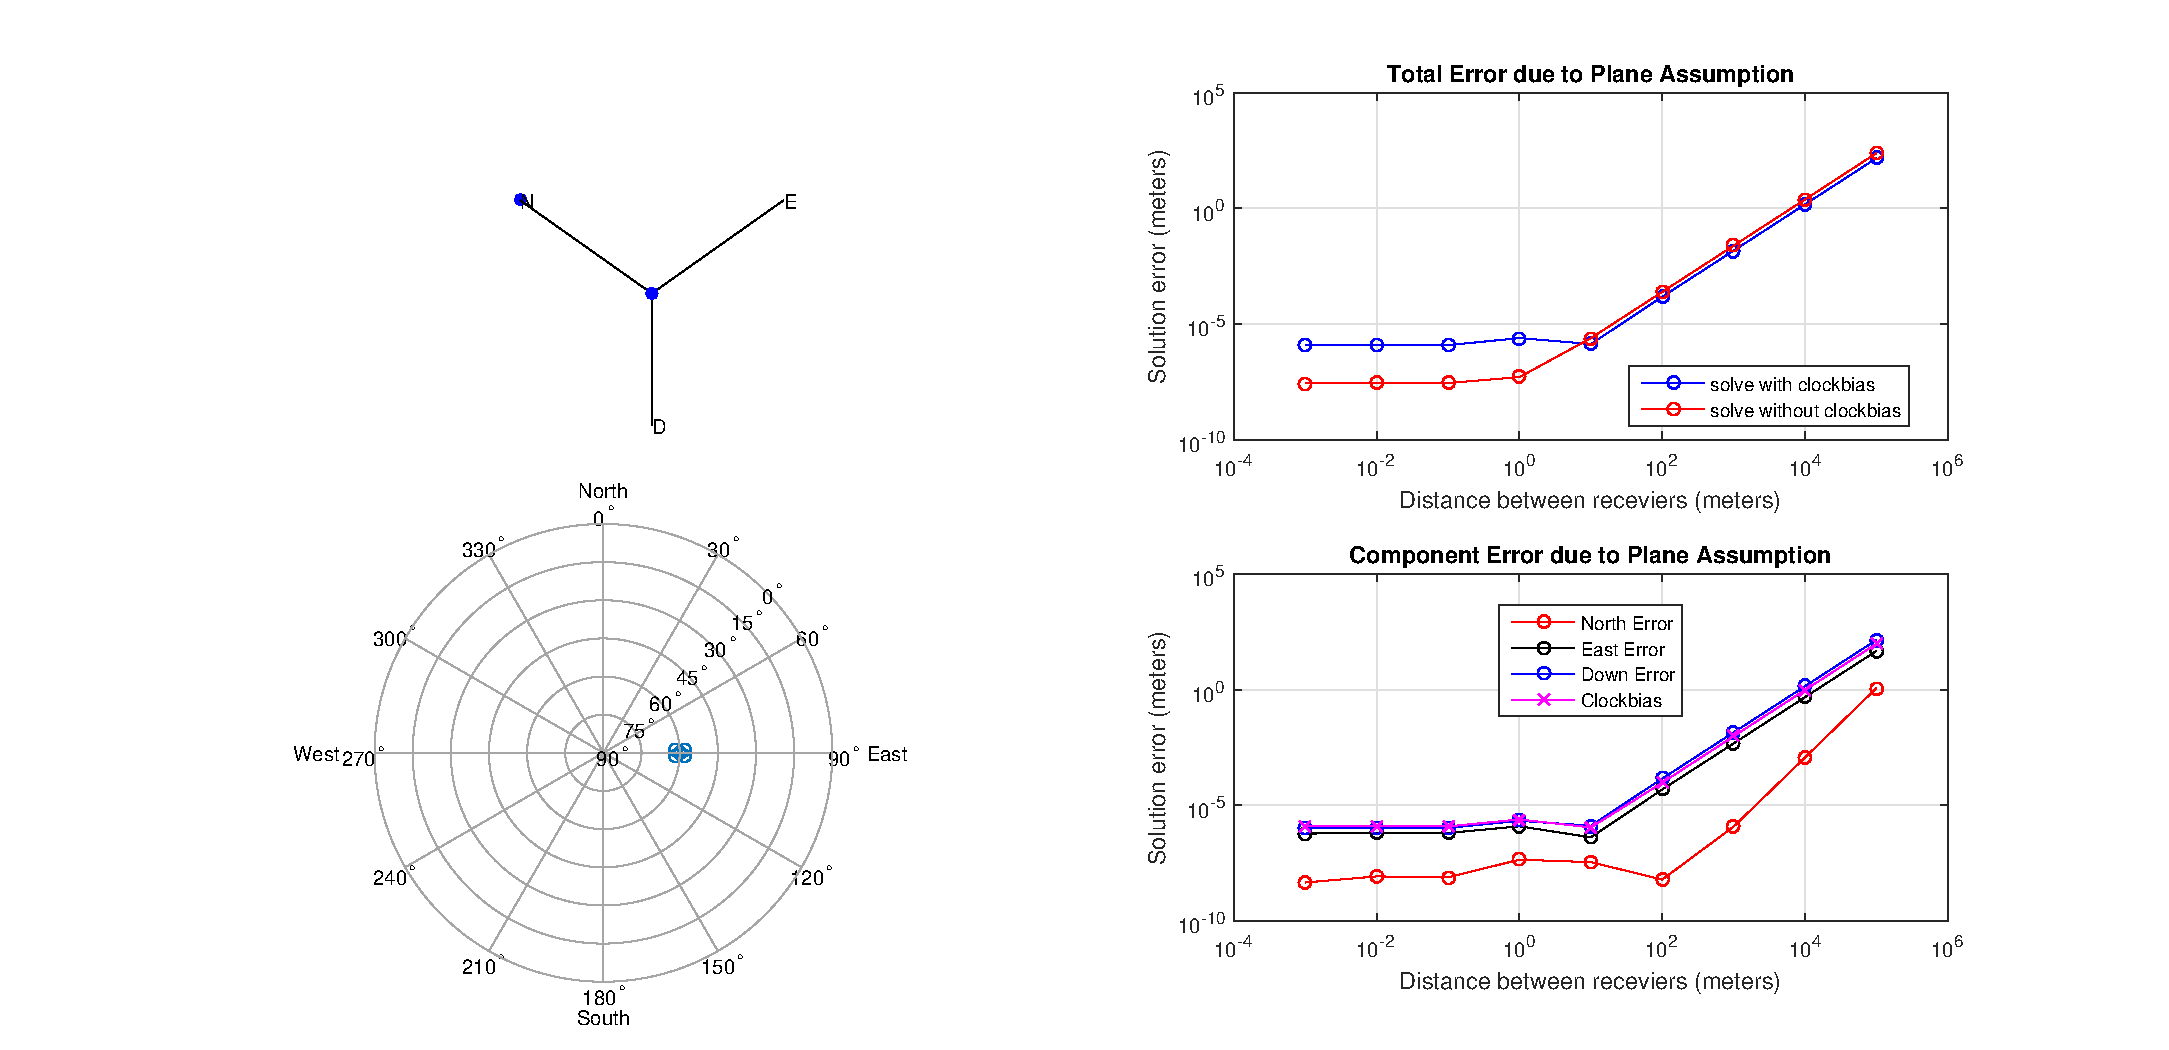
\includegraphics[trim = 3cm 0 0 0,clip,width=\linewidth]{ChapterExperiments/Figures/plane_ALLE_north_9060}
\end{figure}



The configuration of the satellites were also varied. 

NOTE: When the satellites are in a cluster, the planes are very close together with minimal difference between them.
with no errors in the system, the clockbias still went nuts with the constrain (tr-t1) on D
the values of x,y,z are so big for the large differences that a small clockbias is proportionally the minimum
SHOW WITH AND WITHOUT SOLVING FOR CLOCKBIAS
- the excessive clock bias is trying to minimise the error due to the plane assumption



\begin{figure}
\centering
\caption{}
\label{fig:plane_ALLE_north_0075}
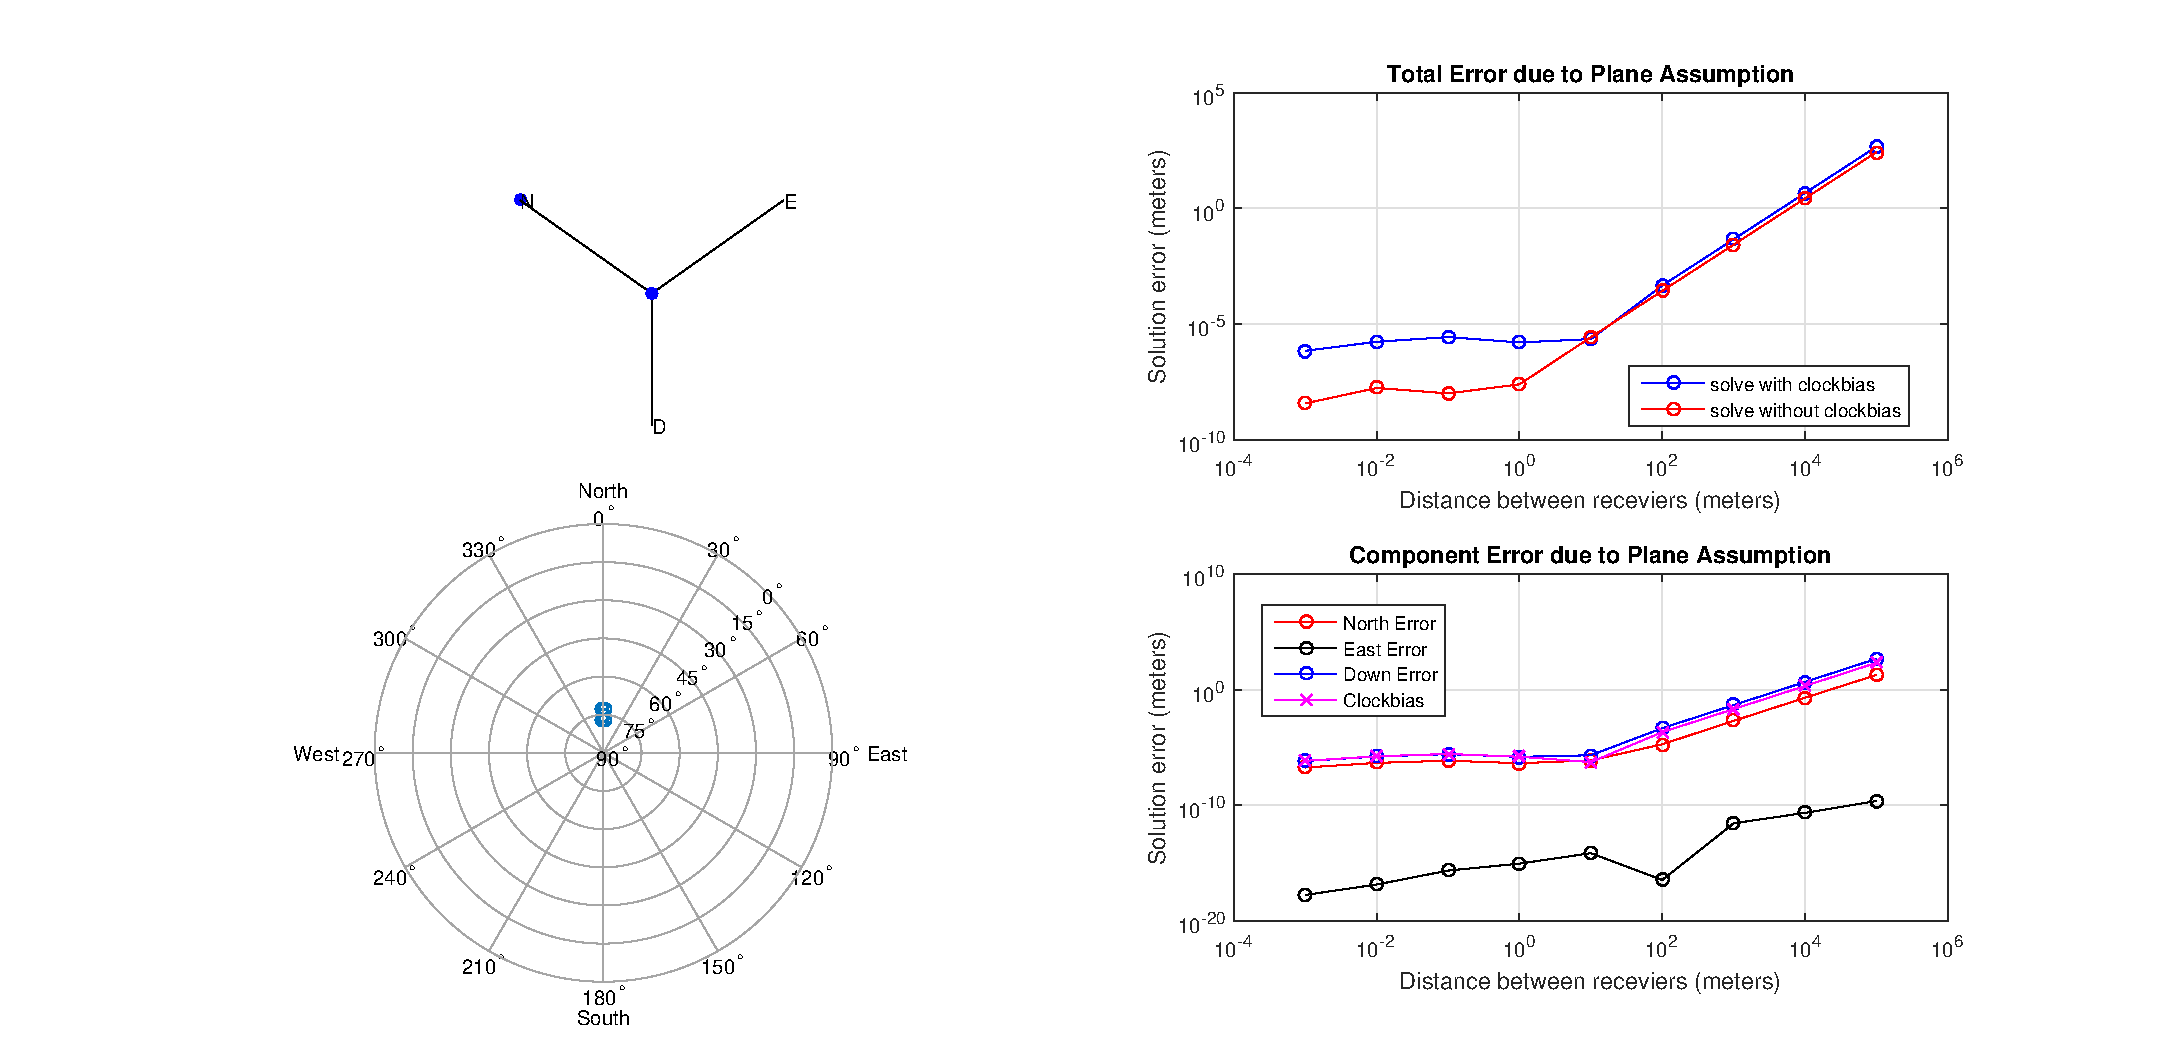
\includegraphics[width=0.7\linewidth]{ChapterExperiments/Figures/plane_ALLE_north_0075}
\end{figure}

%% using main_fn_planesats
\begin{figure}
\centering
\caption{North}
\label{fig:plane_total_north1_pow4}
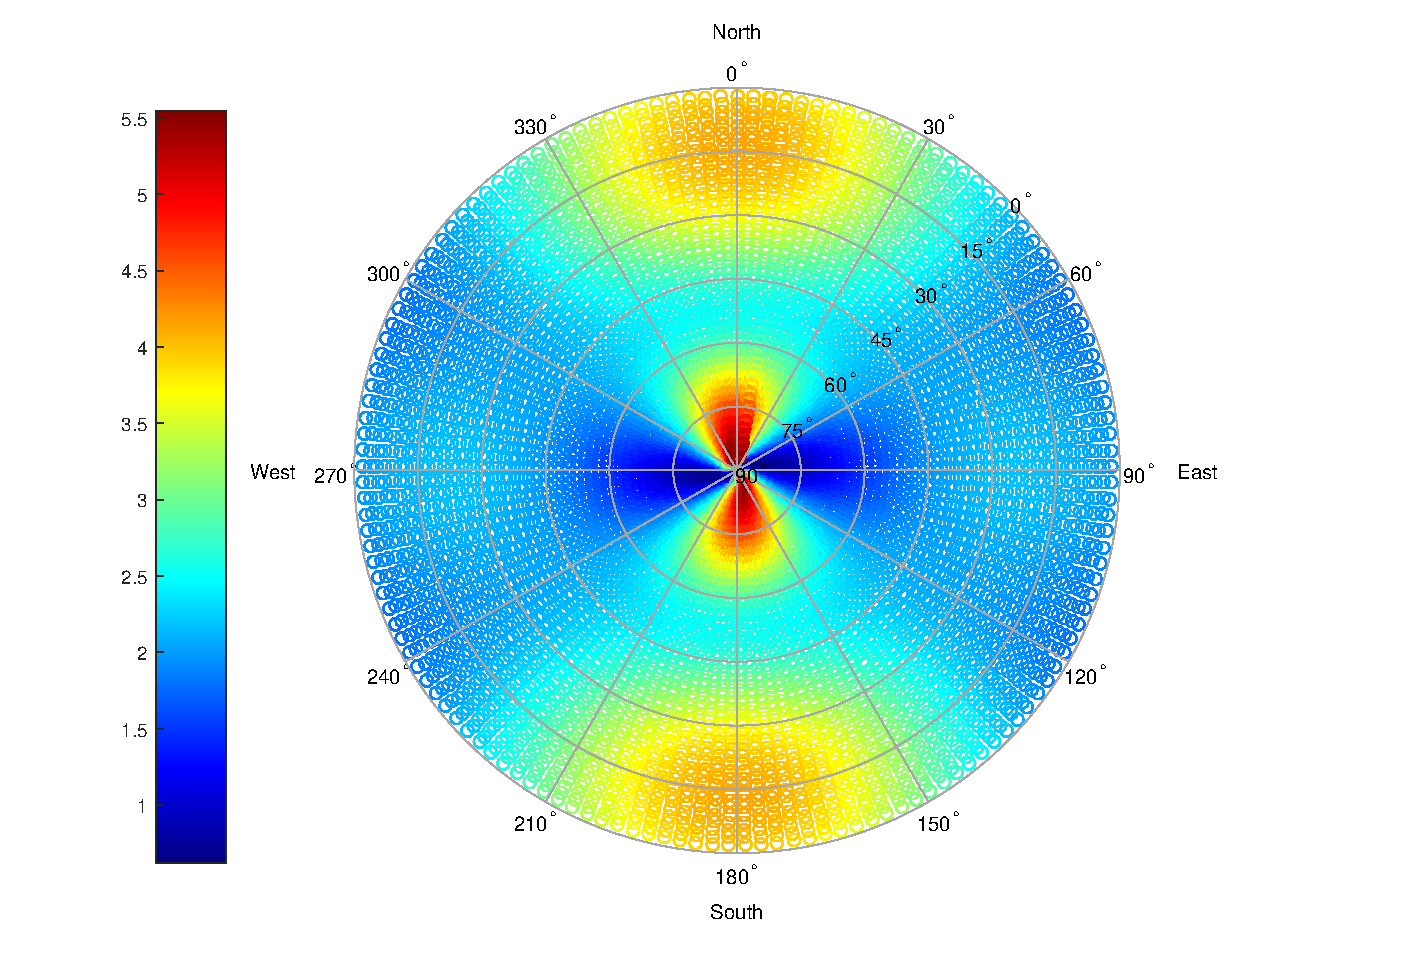
\includegraphics[width=0.7\linewidth]{ChapterExperiments/Figures/plane_total_north1_pow4}
\end{figure}

\begin{figure}
\centering
\caption{East}
\label{fig:plane_total_east_pow4}
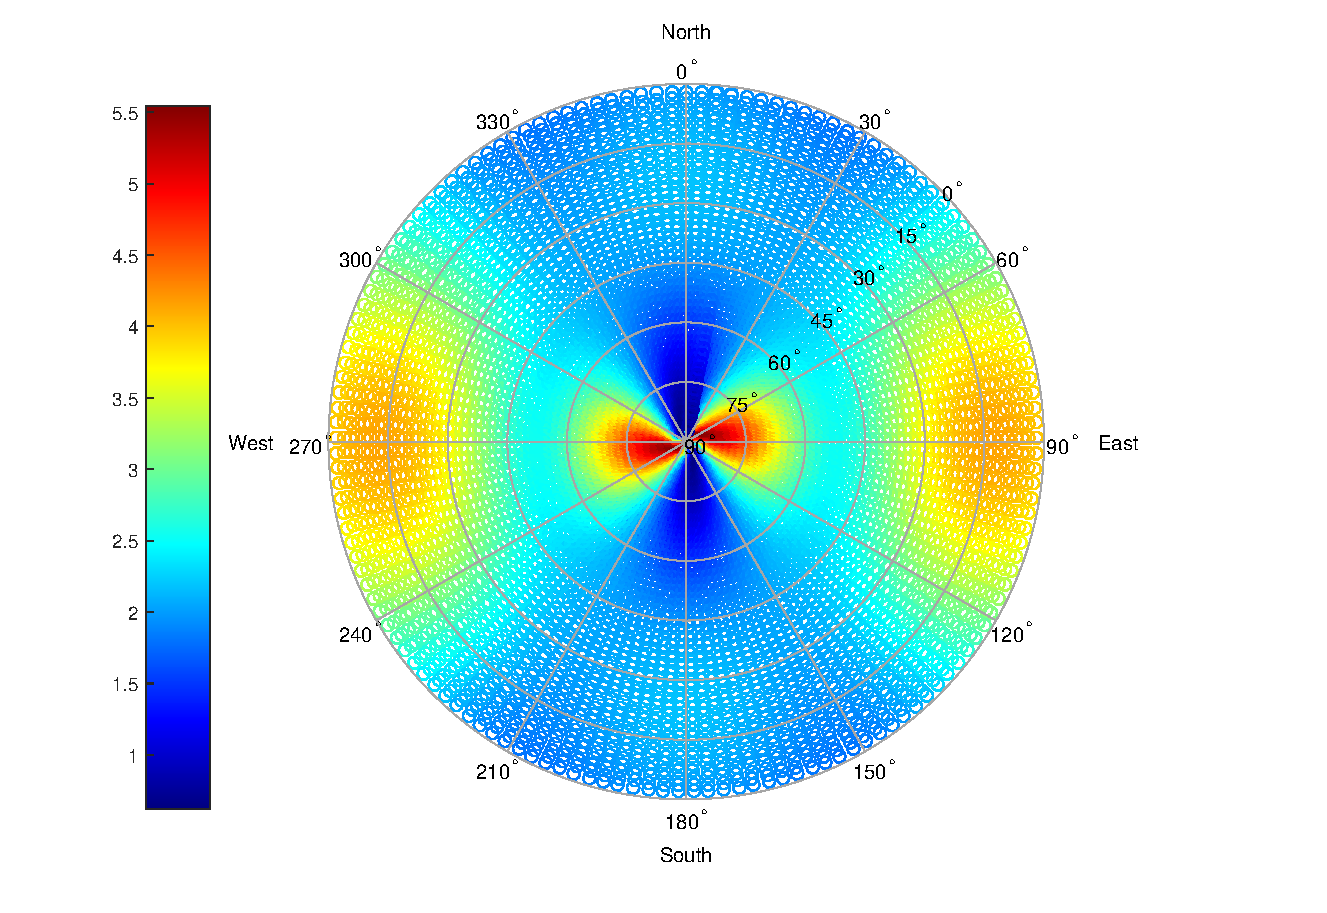
\includegraphics[width=0.7\linewidth]{ChapterExperiments/Figures/plane_total_east_pow4}
\end{figure}

\begin{figure}
\centering
\caption{Down}
\label{fig:plane_total_down_pow4}
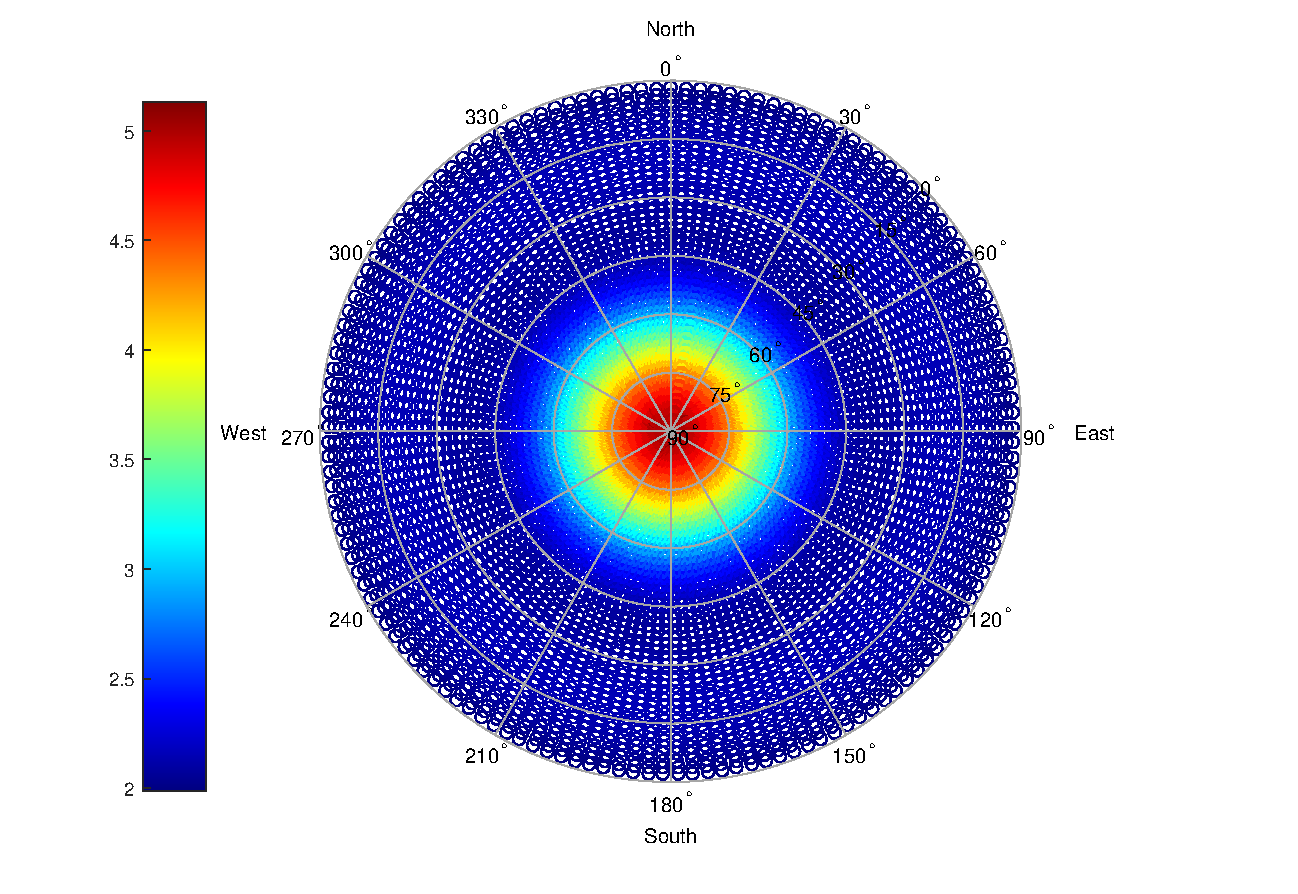
\includegraphics[width=0.7\linewidth]{ChapterExperiments/Figures/plane_total_down_pow4}
\end{figure}

\begin{figure}
\centering
\begin{subfigure}{0.49\textwidth}
\centering
\caption{Config:North, Error:North}
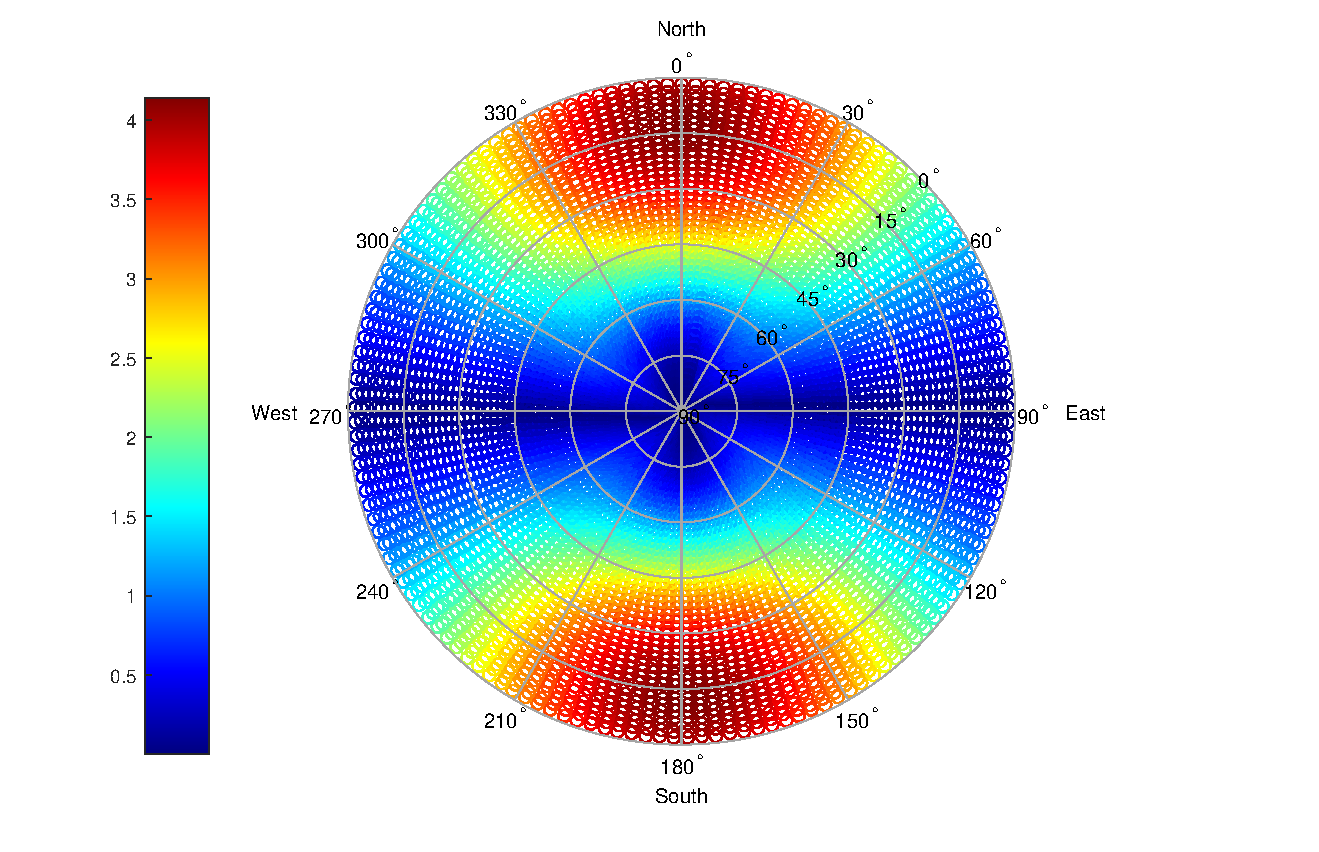
\includegraphics[width =\linewidth]{ChapterExperiments/Figures/plane_Enorth_north_pow4}
\end{subfigure}
\begin{subfigure}{0.49\linewidth}
\centering
\caption{Config:Down, Error:North}
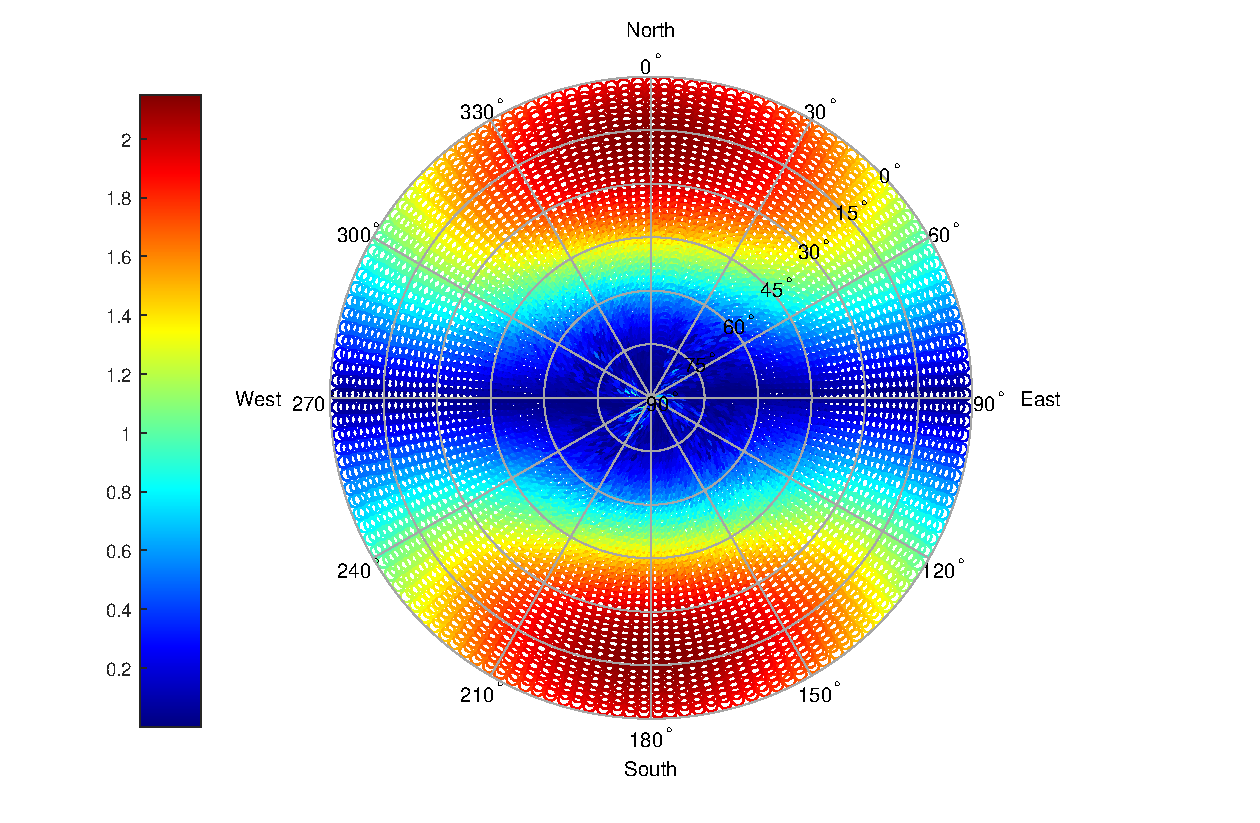
\includegraphics[width = \linewidth]{ChapterExperiments/Figures/plane_Enorth_down_pow4}
\end{subfigure}
\begin{subfigure}{0.49\textwidth}
\centering
\caption{Config:North, Error:East}
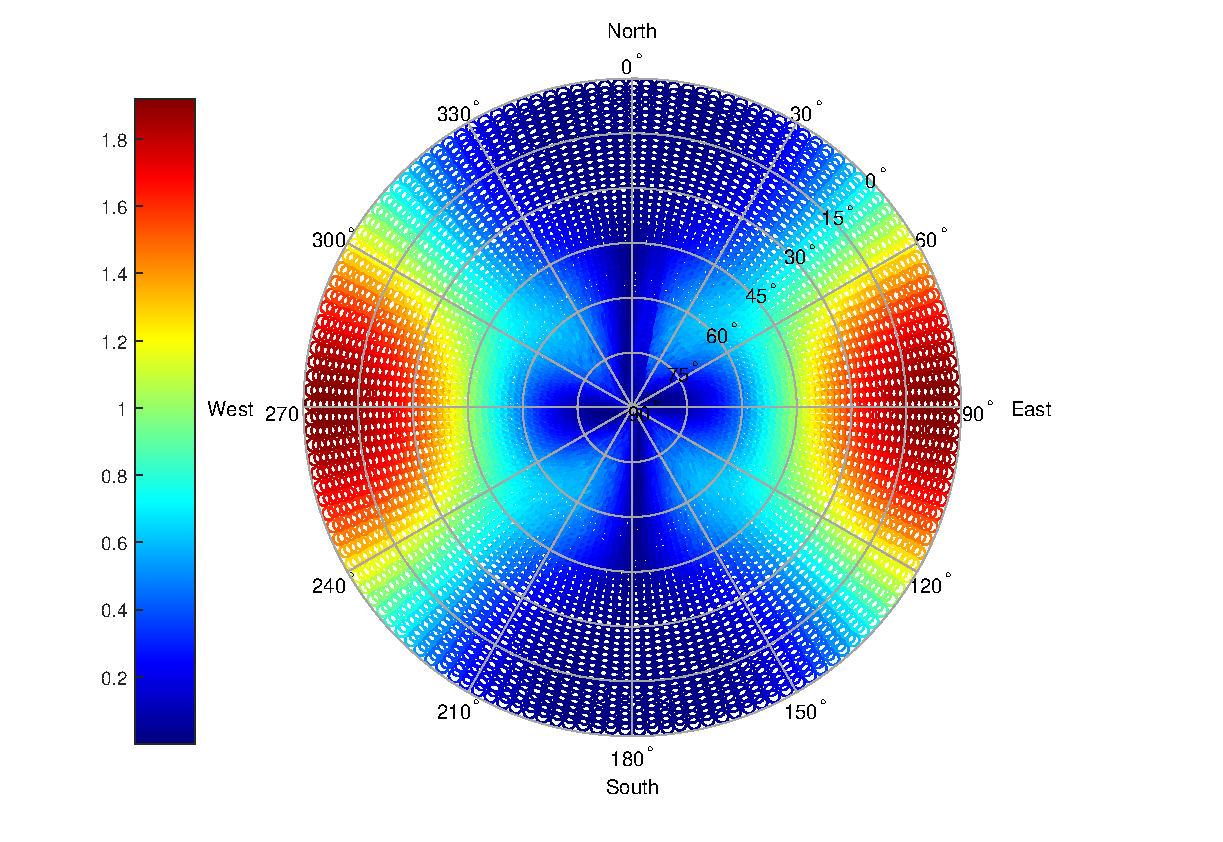
\includegraphics[width =\linewidth]{ChapterExperiments/Figures/plane_Eeast_north_pow4}
\end{subfigure}
\begin{subfigure}{0.49\linewidth}
\centering
\caption{Config:Down, Error:East}
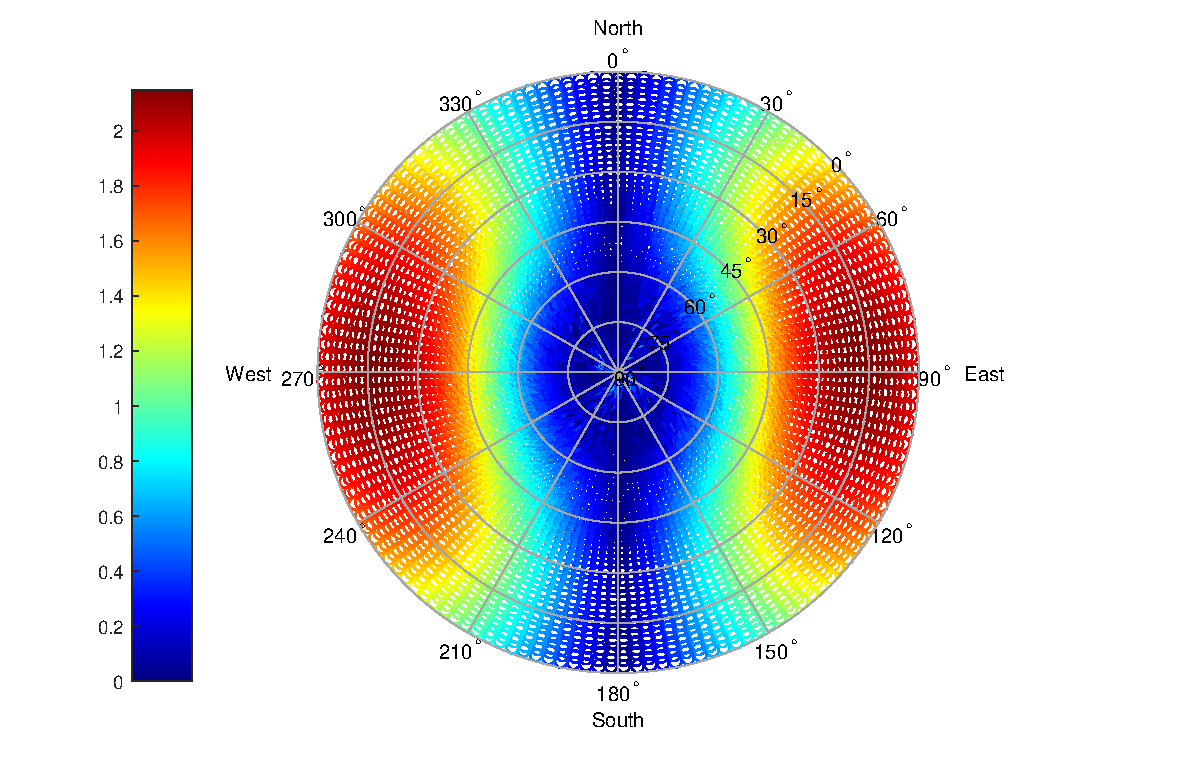
\includegraphics[width = \linewidth]{ChapterExperiments/Figures/plane_Eeast_down_pow4}
\end{subfigure}
\begin{subfigure}{0.49\textwidth}
\centering
\caption{Config:North, Error:Down}
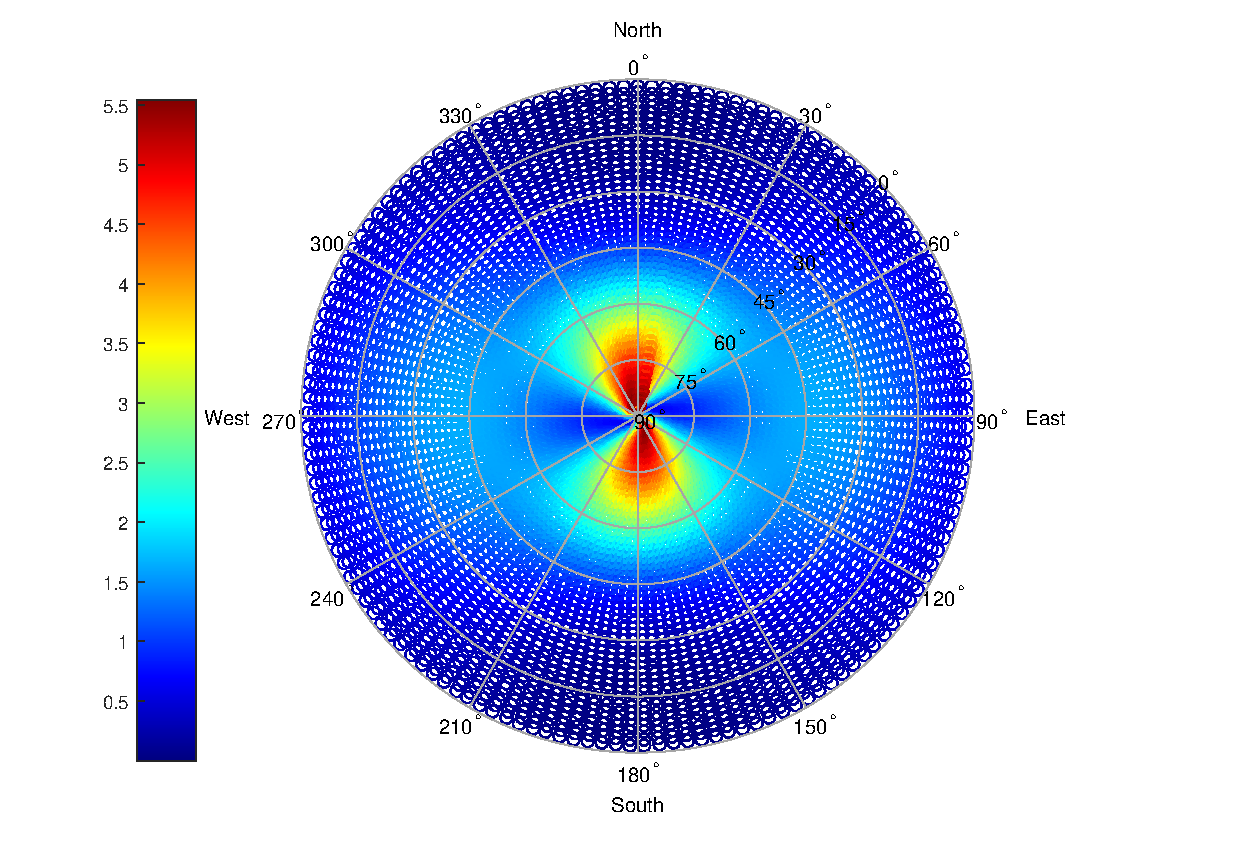
\includegraphics[width =\linewidth]{ChapterExperiments/Figures/plane_Edown_north_pow4}
\end{subfigure}
\begin{subfigure}{0.49\linewidth}
\centering
\caption{Config:Down, Error:Down}
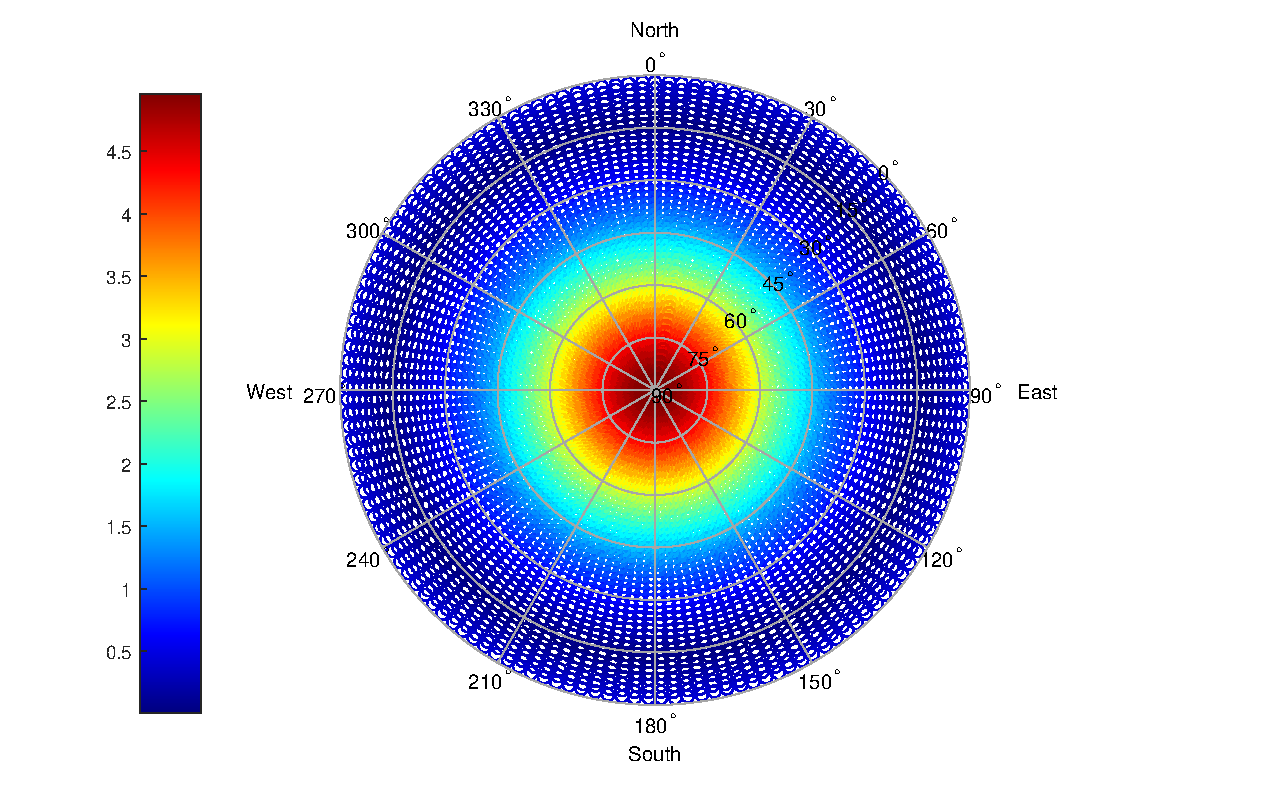
\includegraphics[width = \linewidth]{ChapterExperiments/Figures/plane_Edown_down_pow4}
\end{subfigure}
\end{figure}


%%%%%%%%%%%%%%%%%%%% Conclusions %%%%%%%%%%%%%%%%%%%

- 

			% Chapter 4
%!TEX root = ../thesis.tex

\def\chapdir{./ChapterConclusion}
\chapter{Conclusion}\label{ch:conclusion}

Future work:
Explain how to do it with real systems:
The algorithm is designed with maximum compatibility in mind. 
- any type of receiver that has access to GPS L1 frequency
-



				% Chapter 5

%%==================== List of References ===================================%%
% Note that the List of References goes after the chapters but before the
% appendices. A Bibliography can contain references that are general
% background reading and are not cited in the text. A References or List of
% References section must contain only references that are cited in the text.
% Change to "Bibliography" in commands.tex if you wish and if appropriate.
\cleardoublepage

\begin{singlespace}

    \phantomsection
    \addcontentsline{toc}{chapter}{List of References}  % or "Bibliography"

    % acfrplainnat is a slightly modified version of plainnat from the natbib package.
    % I (AH) removed URLs from the output, since this seems unnecessary or a poorly
    % used field, and adjusted 'misc' to make more sense for the way I used it.

    % Bibliography styles supported by this template are apa-like (default) and ieee
    \bibliographystyle{ieeetrans}
    %\ifthenelse{\equal{\tReferenceStyle}{ieee}}
        %{\bibliographystyle{BibTeX/acfrplainnat}}    % IEEE-like style (or use plainnat)
        %{\bibliographystyle{BibTeX/apalike}}         % APA-like style (or use apalikeAkkaNat)

    \begin{raggedright}     % because you often get ugly whitespace if justified...
        \bibliography{BibTeX/thesis_bib}
    \end{raggedright}

\end{singlespace}

%%==================== Appendices ===========================================%%
% Appendices are almost exactly the same as chapters; the only difference is
% that they come after the \appendix command below.
\appendix 		% Switches from 'Chapter #' to 'Appendix X' chapter titles
%!TEX root = ../Thesis.tex

% This is to set the directory this chapter resides in for images
\def\chapdir{./AppendixSomething}

% Title of this chapter
\chapter{An Example Appendix}\label{ap:something}

As an appendix, this should contain some content that's not really required for the argument in the main body of the thesis, but is clearly relevant and supports the work.

%\input{AppendixSomething/CodeListings}
%\input{AppendixSomething/LargeTables}
%%!TEX root = ../Thesis.tex

\section{Including the PDF of a Relevant Paper}\label{ap:relevantPaper}

Occasionally it may be useful to include whole pages from another document in your thesis, where, for some reason, it is inappropriate or highly inconvenient to convert this into content yourself. This could apply to pages from a technical manual (which would be especially difficult for the average reader to track down), or a highly relevant paper you've published in the field, but not exactly on the thesis topic.

Inclusion of a separate PDF at the page level (rather than just as a floating figure) can be achieved using the \texttt{pdfpages} package\footnote{Please note that there appears to be a namespace clash between the \texttt{pdfpages} and \texttt{graphicx} packages. Including \texttt{pdfpages} \emph{after} \texttt{graphicx} resolves the issue.}. As an example, (three pages of) ``$P \neq NP$'', by Vinay Deolalikar, in its original form are embedded on the following pages.
% Make sure that you cite the paper correctly, and have a very good reason for including it verbatim in this manner!

\includepdf
[
    pages=1-3,      % For all pages, simply use the dash on its own: '-'
    % The pagecommand option adds a header over the top of the included PDF,
    % making it look like part of the thesis document. Here, it has been
    % copied from Thesis/Thesis.tex (so if you change that, you'll need to
    % copy it appropriately)
    pagecommand={\pagestyle{fancyplain}
        \lhead[\fancyplain{}{\thepage}]{\fancyplain{}{\rightmark}}
        \rhead[\fancyplain{}{\leftmark}]{\fancyplain{}{\thepage}}
        \cfoot{}},
    offset=0cm -0.5cm% Move the PDF downwards by 0.5cm.
    % There are many other options to shrink, rotate, etc.
]
{\chapdir/PneqNP}





\end{document}
